\documentclass[a4paper,12pt]{article}

\usepackage[utf8]{inputenc}
\usepackage[margin=1.0in]{geometry}
\usepackage{graphicx}

\title{Examining Image Compression and Reconstruction using Self-Organizing Feature Maps}
\author{.}
\date{March 31st, 2021}

\begin{document}

\maketitle

\begin{abstract}
This paper examines the efficacy of a self-organizing map in compressing and then reconstructing an image from binary file. By analyzing different parameter choices, it is found as a compression tool, this method can be effective; however, in reliability of reproduction, results are mixed depending on parameter choice.
\end{abstract}

\section{Self Organizing Maps}
A self-organizing map (\textbf{SOM}) is a form of artificial neural network which is trained via unsupervised learning---a type of learning where data is unlabeled or the classification of data is not known a priori.

Structured as a lattice of neurons, a SOM takes input vectors and adjusts its own weights such that some part of the lattice closer resembles an input pattern. A SOM is fully connected, that is an input pattern works on every neuron within the network; however, neurons are not interconnected, and as such there are no connections between neurons.

\begin{figure}[h!]
\centering
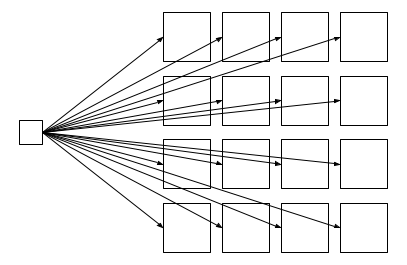
\includegraphics[scale=0.65]{images/som-arch.png}
\caption{Connections between an input and a 4x4 self-organizing map}
\label{fig:somarch}
\end{figure}

In the above \textit{figure 1}, there is a 4x4 SOM and a single input, represented as a vector of some length. When training, the SOM is updated in every neuron based on the characteristics of the input vector and parameters used for training.

\pagebreak

Training is a function of the neighborhood size and learning rate, both being decayed over time as the training algorithm progresses. 

The idea is that a neuron in the lattice is updated such that it becomes "closer" to the given input vector, but of some ratio. For example, a learning rate of 1 will overwrite the neuron with the input vector, whereas a learning rate of 0 will leave the neuron as is: some value inbetween is needed to "blend" neurons together and allow patterns to form.

As for neighborhood radius, while all neurons can be updated in a single pass, the radius of influence an input vector has on the lattice should decrease (decay) over time. Initially, a network may train on the entire network, and by the end it may only train on single neurons at once. The neighborhood radius is around the best-matching unit (\textbf{BMU}), or the position in the lattice where the input vector most resembles (in other words, where its distance to the BMU is smallest).

Each of the weights within the network are updated according to the below rule:

{\Large $$w_i^{t+1} = w_i^t + \phi{(t+1)}\eta{(t+1)}(v - w_i^t)$$}

Where $w_i^t$ represents a given weight at a time $t$, $\phi{}$ is a a neighborhood radius function (where neighborhood decays over time from a default parameter value), $\eta{}$ is a function for learning rate (likewise decaying over time), and $v$ is the current input vector being trained with.

SOMs, over time, exhibit emergent or self patterning behavior, based on network parameters and the characteristics of input data. For example, a common exercise for SOMs is to organize color by hue, as shown in \textit{figure 2} below.

\begin{figure}[h!]
\centering
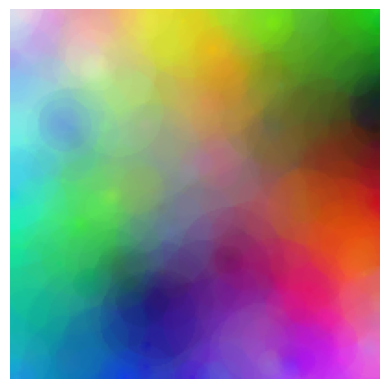
\includegraphics[scale=0.75]{images/euclidean.png}
\caption{A 100x100 self-organizing map used to organize colors}
\label{fig:colormap}
\end{figure}

In this SOM, input vectors consist of 3-tuples corresponding to RGB values. Initially, the lattice is a map of random values, and through reinforced training using the same few color input vectors, patterns emerge. Specifically, "like" colors congregate to "like" colors, but without stark delineation, allowing for a gradient to appear even if a small subset of colors represented in the map are input vectors.

\pagebreak

In a way, new colors are extrapolated from colors within the input vectors and based on their proximity to other, as well as from a stochastic element which means some colors may appear multiple times (consider this SOM has several regions which are broadly "green" which were not grouped together).

\section{Problem Definition}

A SOM can be used for more than color organization: it can be used not only on discrete pixels of RGB values but as well images subdivided into contiguous regions of pixels. For example, as shown in \textit{figure 2}, a 200x200 SOM was used to display a 200x200 grid of colored pixels, instead each neuron in an SOM can be used to display a region of pixels.

Consider the figure below:

\textbf{\begin{figure}[h!]
\centering
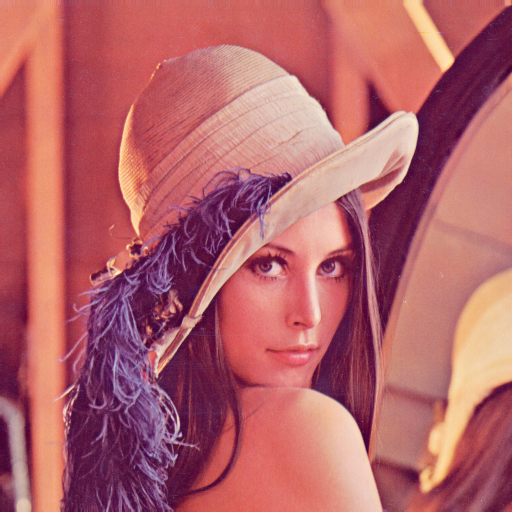
\includegraphics[scale=0.30]{images/lenna.png}
\caption{Sample input image for SOM training}
\label{fig:lenna}
\end{figure}}

While more complicated than organizing RGB pixels, instead something like the above can train an SOM to instead organize contiguous areas of pixels. If this image were subdivided into 128x128 frames (compared to original 512x512 image), to reconstruct this image will need 16 contiguous areas of pixels, and some may be re-used more than once to approximate the original.

\textbf{\begin{figure}[h!]
\centering
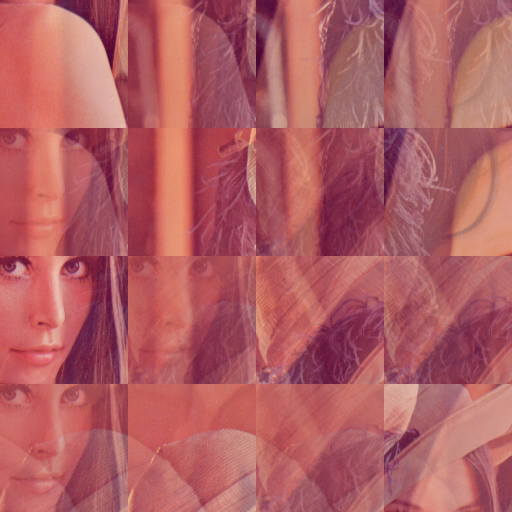
\includegraphics[scale=0.30]{images/lenna_feature_map.png}
\caption{A trained SOM on input image}
\label{fig:lenna_fm}
\end{figure}}

\pagebreak

After training has finished, a SOM is found of subregions of the original image, many of them some blending of multiple subregions. For example, consider the neuron in the 1st column and 2nd row: it is a combination of a face and part of the wall behind the subject.

Then, when reconstructing the image from this SOM, an approximation of the original image can be found:

\textbf{\begin{figure}[h!]
\centering
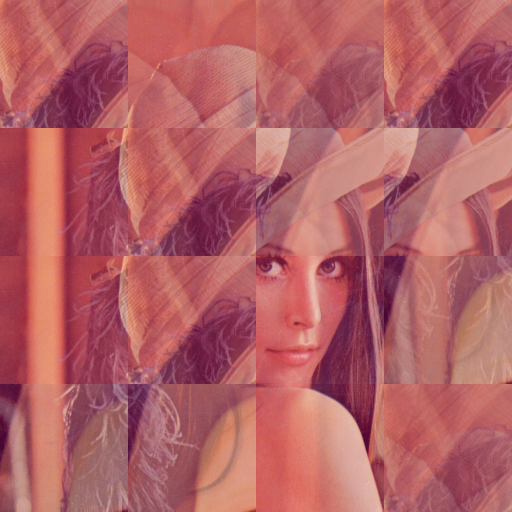
\includegraphics[scale=0.30]{images/lenna_reconstructed_from_memory.png}
\caption{A reconstruction of the input image using the SOM}
\label{fig:lenna_re}
\end{figure}}

While both images are not exactly identical, the gist of the image is preserved. It is known the image is of a human subject, the coloring is correct, and the relative position of features (eg. face, hat) are also preserved. 

However, note that some neurons in the SOM were reused many times because those neurons were a close approximate for the subregion they represent.

This can be taken advantage of: if an image can be reconstructed approximately by re-using subregions of the image many times, the image could be effectively compressed.

The SOM can be used as a "codebook" and indexed to recreate the image. Provided the SOM topology, (eg. dimensions of the network and how many weights exist per neuron), the SOM itself, and a list of indices upon which to reference the SOM, less information can be stored to reconstruct the original image.

\begin{figure}[h!]
\centering
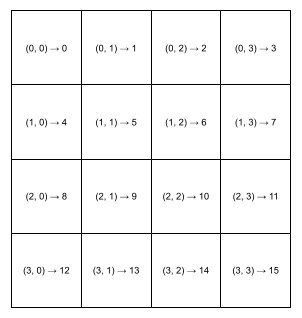
\includegraphics[scale=0.55]{images/indices.png}
\caption{Indices for 4x4 SOM}
\label{fig:indices}
\end{figure}

\pagebreak

\textit{Figure 6} is an illustration of the SOM by coordinates (rows, columns), along with a discrete index. For this 4x4 SOM, 16 neurons exist which can be enumerated $0..15$.

Continuing with this example of a 4x4 SOM and 512x512 image of a woman, the indices in the below figure are found:

\begin{figure}[h!]
\centering
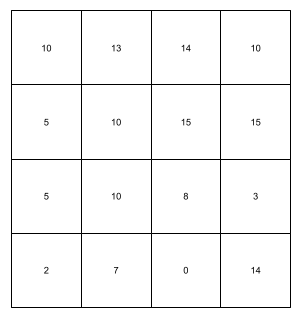
\includegraphics[scale=0.55]{images/recon_indices.png}
\caption{Indices for reconstructed image}
\label{fig:lindices}
\end{figure}

Of note is one index was re-used four times, three were used twice, and six were not used at all. In fact, of the sixteen indices represented, only ten were needed to recreate the image, therefore only about $63\%$ of the information is needed to approximate the original.

This suggests that SOMs could be used as a form of compression since less data needs to be stored to represent images. The problem, however, is in its efficacy as a compression algorithm as while it can approximate images, it is not a perfect recreation.

\section{Experimental Setup}

Implemented was a variable-size SOM which took an input in form of RGB .PNG image, divided the input into input vectors, and then was trained using these input vectors. Once training concluded, a codebook was formed from neurons of the SOM and placed into a binary file along with the BMUs that would best reconstruct the original image using only this information.

Multiple tests were performed, including varying the network size, input vector size (as a function of frame slices of input image), metric space used for distance calculations, and number of epochs. Indirectly, the number of epochs also impacts the learning rate and neighborhood radius for training.

The network size denotes how many neurons exist within the network, with the tests conducted training a 4x4, 8x8, and 16x16 network to determine its import on performance. Likewise, the frame size denotes the size of contiguous areas used to train the network.

The metric space, between Euclidean, Manhattan, and Chebyshev, is simply the difference of distance function used to determine the BMU position in the SOM as well as determining which index in the SOM codebook to use for image recreation.

The amount of epochs determines how long training should occur for as well as how quickly the neighborhood radius and learning rates decay.

\pagebreak

Twelve tests are performed, testing each parameter in three different scenarios:

\begin{table}[h!]
\centering
\begin{tabular}{c|c|c|c|c|}
\cline{2-5}
\multicolumn{1}{l|}{} & \textbf{Network Size} & \textbf{Frame Size} & \textbf{Metric Space} & \textbf{Epochs} \\ \hline
\multicolumn{1}{|c|}{\textit{Test 1}} & 4x4 & 4x4 & Euclidean & 50 \\ \hline
\multicolumn{1}{|c|}{\textit{Test 2}} & 8x8 & 8x8 & Manhattan & 200 \\ \hline
\multicolumn{1}{|c|}{\textit{Test 3}} & 16x16 & 16x16 & Chebyshev & 500 \\ \hline
\end{tabular}
\caption{Test parameters}
\end{table}

For all tests, the learning rate is locked at $0.35$ because it created either the most visually pleasing outputs or provided the lowest error in reproduction. Similarly, the initial neighborhood radius is locked at the width of the network itself. Both of these parameters still decay according to the number of epochs.

The error measure is mean squared error (\textbf{MSE}), which denotes how dissimilar an original image is compared to its reconstruction (closer to zero means closer in similarity/less error in reproduction). 

Not only this, but filesizes of binary files compared to their originals is examined. This is given as a percentage of original filesize, with positive meaning a successful compression, and negative meaning an unsuccessful compression.

\begin{figure}[h!]
\centering
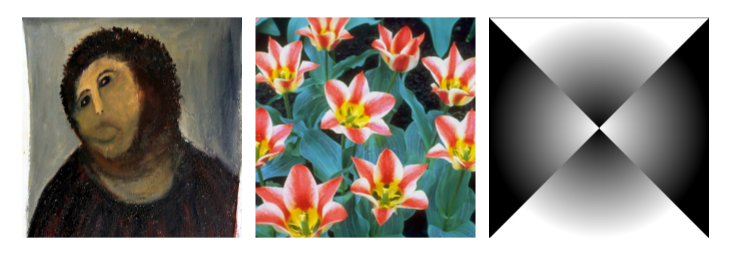
\includegraphics[scale=0.50]{images/images.png}
\caption{Sample inputs: `eccemono`, `tulips`, `pattern`}
\label{fig:images}
\end{figure}

Three image samples are used: `eccemono`, a color painting, `tulips`, a color photograph, and `pattern`, a grayscale image of a geometric gradient.

All tests are performed five times with the mean of MSE being tabulated. Compression size is consistent between executions as it is a function of the parameters and not stochastic.

\section{Experimental Results}

Since some parameters are being tested while other parameters are also being tested later, some arbitrary value for those parameters must be chosen. Since results should be generally good and only be indicative of the parameter being tests, these are set as values that are known to be generally good. This way results closer show the impact of the tested parameter rather than a combination of parameters.

\pagebreak

\subsection{Network Size}

The first test is considering the network size. Three sizes are tested: 4x4, 8x8, and 16x16. This tests compares the MSE and compression ability of each network size.

\begin{table}[h!]
\footnotesize
\centering
\begin{tabular}{c|c|c|c|c|c|c|}
\cline{2-7}
 & \multicolumn{2}{c|}{\textbf{4x4}} & \multicolumn{2}{c|}{\textbf{8x8}} & \multicolumn{2}{c|}{\textbf{16x16}} \\ \cline{2-7} 
 & \textit{MSE} & \textit{Size} & \textit{MSE} & \textit{Size} & \textit{MSE} & \textit{Size} \\ \hline
\multicolumn{1}{|c|}{\textit{`eccemono`}} & 2046.77 & 4\% & 1516.17 & 9\% & 1541.8 & 28\% \\ \hline
\multicolumn{1}{|c|}{\textit{`tulips`}} & 5065.11 & 5\% & 4069.33 & 11\% & 3957.39 & 36\% \\ \hline
\multicolumn{1}{|c|}{\textit{`pattern`}} & 4371.19 & 26\% & 4326.4 & 55\% & 3886.68 & -74\% \\ \hline
\end{tabular}
\caption{Results for Network Size test}
\end{table}

From above, it can be deduced that a smaller network has a reduced ability to reproduce an image, leading to higher error, but has better compression ability. Of note is `eccemono` is able to be compressed to 4\% of its original filesize; conversely, for `pattern`, a 16x16 network actually increased the file size to nearly double its original.

\subsection{Frame Size}

The second test is to vary the frame sizing from 4x4, 8x8, and 16x16 to likewise compare efficiency in compression and ability to reproduce the original image.

\begin{table}[h!]
\footnotesize
\centering
\begin{tabular}{c|c|c|c|c|c|c|}
\cline{2-7}
 & \multicolumn{2}{c|}{\textbf{4x4}} & \multicolumn{2}{c|}{\textbf{8x8}} & \multicolumn{2}{c|}{\textbf{16x16}} \\ \cline{2-7} 
 & \textit{MSE} & \textit{Size} & \textit{MSE} & \textit{Size} & \textit{MSE} & \textit{Size} \\ \hline
\multicolumn{1}{|c|}{\textit{`eccemono`}} & 1360.02 & 12\% & 1341.76 & 9\% & 2573.36 & 25\% \\ \hline
\multicolumn{1}{|c|}{\textit{`tulips`}} & 1784.12 & 15\% & 4159.78 & 11\% & 7083.97 & 33\% \\ \hline
\multicolumn{1}{|c|}{\textit{`pattern`}} & 1857.22 & 73\% & 4049.62 & 55\% & 7782.66 & -61\% \\ \hline
\end{tabular}
\caption{Results for Frame Size test}
\end{table}

Looking at these results suggest a smaller frame size leads to a better reproduction, with 16x16 in particular performing poorly for all images tested. Interestingly, for each image, going from 4x4 to 8x8 lead to better compression, but from 8x8 to 16x16 lead to much worse compression, even worse than 4x4. This suggests there is a "sweet spot" for frame size where compression ability is maximized.

\subsection{Metric Space}

The third test compares the metric space used for distance calculations.

\begin{table}[h!]
\footnotesize
\centering
\begin{tabular}{c|c|c|c|c|c|c|}
\cline{2-7}
 & \multicolumn{2}{c|}{\textbf{Euclidean}} & \multicolumn{2}{c|}{\textbf{Manhattan}} & \multicolumn{2}{c|}{\textbf{Chebyshev}} \\ \cline{2-7} 
 & \textit{MSE} & \textit{Size} & \textit{MSE} & \textit{Size} & \textit{MSE} & \textit{Size} \\ \hline
\multicolumn{1}{|c|}{\textit{`eccemono`}} & 561.25 & 11\% & 613.63 & 11\% & 1600.68 & 11\% \\ \hline
\multicolumn{1}{|c|}{\textit{`tulips`}} & 892.83 & 15\% & 996.02 & 15\% & 1900.84 & 15\% \\ \hline
\multicolumn{1}{|c|}{\textit{`pattern`}} & 1727.83 & 73\% & 1816.31 & 73\% & 2017.77 & 73\% \\ \hline
\end{tabular}
\caption{Results for Metric Space test}
\end{table}

These results suggest the metric space used does not have a large impact on either compression or accuracy, except in the case of Chebyshev metrics which reduces accuracy.

\pagebreak

\subsection{Epochs}

The final test compares the impact the number of epochs used for training has on accuracy and compression ability.

\begin{table}[h!]
\footnotesize
\centering
\begin{tabular}{c|c|c|c|c|c|c|}
\cline{2-7}
 & \multicolumn{2}{c|}{\textbf{50}} & \multicolumn{2}{c|}{\textbf{200}} & \multicolumn{2}{c|}{\textbf{500}} \\ \cline{2-7} 
 & \textit{MSE} & \textit{Size} & \textit{MSE} & \textit{Size} & \textit{MSE} & \textit{Size} \\ \hline
\multicolumn{1}{|c|}{\textit{`eccemono`}} & 2285.43 & 11\% & 1329.47 & 11\% & 833.66 & 11\% \\ \hline
\multicolumn{1}{|c|}{\textit{`tulips`}} & 3033.25 & 15\% & 1876.57 & 15\% & 902.88 & 15\% \\ \hline
\multicolumn{1}{|c|}{\textit{`pattern`}} & 1869.72 & 73\% & 2199.76 & 73\% & 1862.1 & 73\% \\ \hline
\end{tabular}
\caption{Results for Epoch test}
\end{table}

The amount of training epochs has a strong impact on accuracy of reproduction but does not affect compression ability, as compressed file size is a function of topology and frame sizing than the number of epochs.

\section{Results Summary}

On comparing the found results, some generalizations can be made about the parameter choices.

Network size determines how many distinct frames can exist in the image reproduction and a larger network means less frame re-use is needed. As a consequence, two things occur: the compression is weaker, as the included codebook needs to be larger, but accuracy in reproduction is increased. A reconstruction of original image is more likely to be accurate the larger the network is. Between network sizes used, the larger a network is, the better an image can be reproduced at the consequence of poorer compression.

Frame size determines how large subregions exist in the final image. On the low end, as you approach pixel sizes, accuracy increases and compression efficiency decreases. However, it is not the inverse were the frame size to increase linearly: there is a "sweet spot" where accuracy and compression ability is maximized, although this is dependent on the type of image provided and the threshold is very small. For the frame sizes tests, it is situation specific whether 4x4 or 8x8 outperforms another, but 16x16 leads to poor results for both measure.

Metric space, contrastingly, has no affect on compression efficacy but does in image reproduction. Euclidean metric space was ideal although Manhattan is not far behind. Chebyshev metric space was found to be impractical as perform was much worse than the other metrics used.

The number of epochs used to train the network is linearly related to the effect in reconstructing images, although it had no impact on compression. As the network is trained longer, it is able to better approximate the original image, and therefore it is advised to train for as long as reasonable. For the tests conducted, 500 epochs was sufficient to reach a small enough MSE to consider the image subjectively reproduced.

Three different types of images were tested: a painting, a photograph, and geometry. The geometric shape, while able to be compressed for some tests, is much less efficient than the other types of images tested.

\pagebreak

\begin{figure}[h!]
\centering
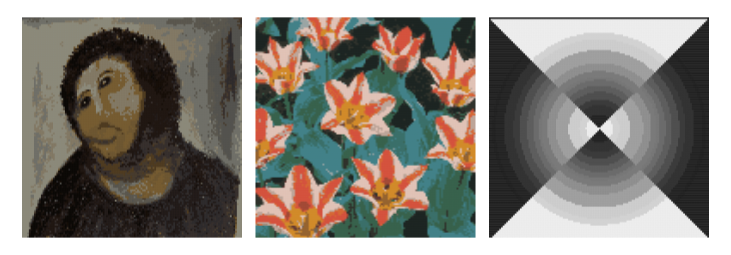
\includegraphics[scale=0.50]{images/bestsize.png}
\caption{Best reproductions based on compression ability}
\label{fig:bestsize}
\end{figure}

Comparing the reproduced images to the original based on compression ability (minimizing filesize), all three are still somewhat resembling the originals albeit with loss of color depth and loss of definition. On average, prioritizing compression ability resulted in binary file sizes approximately 12\% of the original. Consider \textit{figure 9}.

\begin{figure}[h!]
\centering
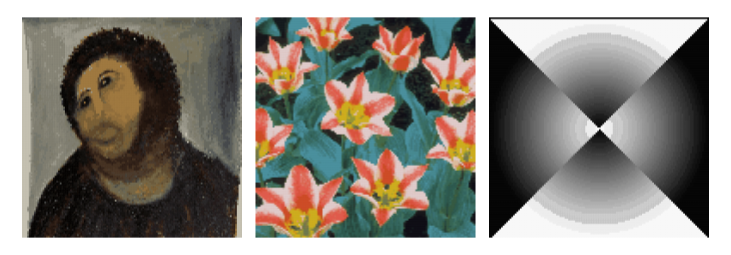
\includegraphics[scale=0.50]{images/bestmse.png}
\caption{Best reproductions based on MSE}
\label{fig:bestmse}
\end{figure}

However, were MSE to be prioritized---that is, that the goal of the algorithm is to reproduce the image as close as possible---the images closer resemble the originals. When considering \textit{figure 10} below, colors are more vibrant than in \textit{figure 9}, and there exists more detail. However, it is still not an exact reduplication of the original image, although it is close.

\section{Conclusion}

Upon examining the efficacy of SOMs in compressing images, some promise is shown with regards to shrinking file sizes although reproduction of original images can be difficult as a fair amount of information is lost in compression.

If perfect reproduction is a requirement for an image compression format, SOM may be inadequate, as in all tests, reproduction is poor. However, if only approximations of images is needed, this method shows promise with on average 12\% of original information being required to reproduce images.

For applications like academic papers, or if images are to be shrinked further, the loss of detail may not matter. But, for large format printing or image processing, SOM is an inappropriate method. There is still opportunity to fine tune, however, as reproduction is possible, it just requires a large enough network, and small enough frame sizing.

\end{document}
